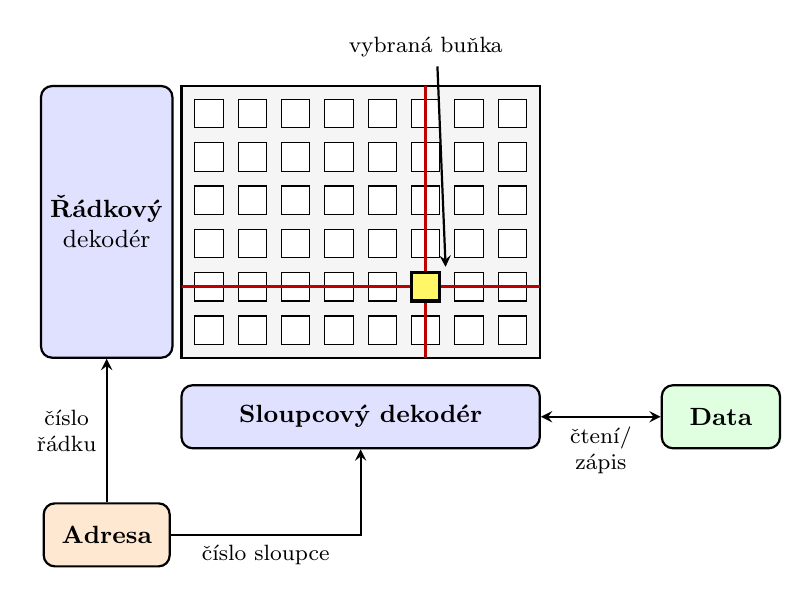
\begin{tikzpicture}[
    x=1cm, y=1cm,
    >=stealth,
    every node/.style={font=\small},
    box/.style={
        draw,
        thick,
        rounded corners,
        align=center
    },
    lab/.style={font=\footnotesize, align=center},
    arr/.style={->, thick},
    cell/.style={draw, minimum size=0.36cm, inner sep=0pt, fill=white},
    hilite/.style={draw, very thick, minimum size=0.36cm, inner sep=0pt, fill=yellow!60}
]

    % Vybraná buňka: řádek 1 (počítáno odspodu od 0), sloupec 5
    \def\selrow{1}
    \def\selcol{5}

    % Matice paměťových buněk 6 x 8
    \draw[thick, fill=gray!8] (-0.35,-0.35) rectangle (4.2,3.1);
    \foreach \r in {0,...,5}{
        \foreach \c in {0,...,7}{
            \node[cell] at (0.55*\c, 0.55*\r) {};
        }
    }

    % Aktivní řádek a sloupec
    \draw[red!75!black, very thick] (-0.35,0.55*\selrow) -- (4.2,0.55*\selrow);
    \draw[red!75!black, very thick] (0.55*\selcol,-0.35) -- (0.55*\selcol,3.1);
    \node[hilite] (sel) at (0.55*\selcol,0.55*\selrow) {};

    \node[lab, anchor=south] (sellab) at (0.55*\selcol,3.35) {vybraná buňka};
    \draw[->, thick] (sellab.south) ++(0.15,0) -- ([xshift=1.5pt,yshift=1.5pt]sel.north east);

    % Řádkový dekodér vlevo
    \node[box, fill=blue!12, minimum width=1.6cm, minimum height=3.45cm] (rowdec) at (-1.3,1.375)
        {\textbf{Řádkový}\\ dekodér};

    % Sloupcový dekodér pod maticí
    \node[box, fill=blue!12, minimum width=4.55cm, minimum height=0.8cm] (coldec) at (1.925,-1.1)
        {\textbf{Sloupcový dekodér}};

    % Adresa vlevo dole
    \node[box, fill=orange!18, minimum width=1.6cm, minimum height=0.8cm] (addr) at (-1.3,-2.6)
        {\textbf{Adresa}};

    \draw[arr] (addr.north) -- node[left, lab] {číslo\\řádku} (rowdec.south);
    \draw[arr] (addr.east) -| node[pos=0.25, below, lab] {číslo sloupce} (coldec.south);

    % Data
    \node[box, fill=green!12, minimum width=1.5cm, minimum height=0.8cm] (data) at (6.5,-1.1)
        {\textbf{Data}};
    \draw[<->, thick] (coldec.east) -- node[below, lab] {čtení/\\zápis} (data.west);

\end{tikzpicture}
